\documentclass[10pt]{article}
%$Id: macro.tex,v 1.10 2004/12/08 13:38:58 acary Exp $


%\usepackage{a4wide}
\textheight 25cm
\textwidth 16.5cm
\topmargin -1cm
%\evensidemargin 0cm
\oddsidemargin 0cm
\evensidemargin0cm
\usepackage{layout}


\usepackage{amsmath}
\usepackage{amssymb}
\usepackage{minitoc}
%\usepackage{glosstex}
\usepackage{colortbl}
\usepackage{hhline}
\usepackage{longtable}

%\usepackage{glosstex}
%\def\glossaryname{Glossary of Notation}
\def\listacronymname{Acronyms}

\usepackage[outerbars]{changebar}\setcounter{changebargrey}{20}
%\glxitemorderdefault{acr}{l}

%\usepackage{color}
\usepackage{graphicx,epsfig}
\graphicspath{{figure/}}
\usepackage[T1]{fontenc}
\usepackage{rotating}

%\usepackage{algorithmic}
%\usepackage{algorithm}
\usepackage{ntheorem}
\usepackage{natbib}


%\renewcommand{\baselinestretch}{2.0}
\setcounter{tocdepth}{2}     % Dans la table des matieres
\setcounter{secnumdepth}{3}  % Avec un numero.



\newtheorem{definition}{Definition}
\newtheorem{lemma}{Lemma}
\newtheorem{claim}{Claim}
\newtheorem{remark}{Remark}
\newtheorem{assumption}{Assumption}
\newtheorem{example}{Example}
\newtheorem{conjecture}{Conjecture}
\newtheorem{corollary}{Corollary}
\newtheorem{OP}{OP}
\newtheorem{problem}{Problem}
\newtheorem{theorem}{Theorem}


\newcommand{\CC}{\mbox{\rm $~\vrule height6.6pt width0.5pt depth0.25pt\!\!$C}}
\newcommand{\ZZ}{\mbox{\rm \lower0.3pt\hbox{$\angle\!\!\!$}Z}}
\newcommand{\RR}{\mbox{\rm $I\!\!R$}}
\newcommand{\NN}{\mbox{\rm $I\!\!N$}}

\newcommand{\Mnn}{\mathcal M^{n\times n}}
\newcommand{\Mnp}[2]{\ensuremath{\mathcal M^{#1\times #2}}}



\newcommand{\Frac}[2]{\displaystyle \frac{#1}{#2}}

\newcommand{\DP}[2]{\displaystyle \frac{\partial {#1}}{\partial {#2}}}

% c++ variables writting
\newcommand{\varcpp}[1]{\textit{#1}}
% itemize
\newcommand{\bei}{\begin{itemize}}
\newcommand{\ei}{\end{itemize}}

\newcommand{\ie}{i.e.}
\newcommand{\eg}{e.g.}
\newcommand{\cf}{c.f.}
\newcommand{\putidx}[1]{\index{#1}\textit{#1}}

\def\Er{{\rm I\! R}}
\def\En{{\rm I\! N}} 
\def\Ec{{\rm I\! C}}
 
\def\zc{\hat{z}}
\def\wc{\hat{w}}

\font\tete=cmr8 at 8 pt
\font\titre= cmr12 at 20 pt 
\font\titregras=cmbx12 at 20 pt

%----------------------------------------------------------------------
%                  Modification des subsubsections
%----------------------------------------------------------------------
\makeatletter
\renewcommand\thesubsubsection{\thesubsection.\@alph\c@subsubsection}
\makeatother

%----------------------------------------------------------------------
%             Redaction note environnement
%----------------------------------------------------------------------
\makeatletter
\theoremheaderfont{\scshape}
\theoremstyle{marginbreak}
\theorembodyfont{\upshape}
%\newtheorem{rque}{\bf Remarque}[chapter]
%\newtheorem{rque1}{\bf \fsc{Remarque}}[chapter] !!! \fsc est une commande french
\newtheorem{ndr1}{\textbf{\textsc{Redaction note}}}[section]

\newenvironment{ndr}%
{%
\tt
%\centerline{---oOo---}
\noindent\begin{ndr1}%
}%
{%
\begin{flushright}%
%\vspace{-1.5em}\ding{111}
\end{flushright}%
\end{ndr1}%
%\centerline{---oOo---}
}

\makeatother

%----------------------------------------------------------------------
%             Redaction note environnement V.ACARY
%----------------------------------------------------------------------
\makeatletter
\theoremheaderfont{\scshape}
\theoremstyle{marginbreak}
\theorembodyfont{\upshape}
%\newtheorem{rque}{\bf Remarque}[chapter]
%\newtheorem{rque1}{\bf \fsc{Remarque}}[chapter] !!! \fsc est une commande french
\newtheorem{ndr1va}{\textbf{\textsc{Redaction note V. ACARY}}}[section]

\newenvironment{ndrva}%
{%
\tt
%\centerline{---oOo---}
\noindent\begin{ndr1va}%
}%
{%
\begin{flushright}%
%\vspace{-1.5em}\ding{111}
\end{flushright}%
\end{ndr1va}%
%\centerline{---oOo---}
}

\makeatother
%----------------------------------------------------------------------
%             Redaction note environnement V.ACARY
%----------------------------------------------------------------------
\makeatletter
\theoremheaderfont{\scshape}
\theoremstyle{marginbreak}
\theorembodyfont{\upshape}
%\newtheorem{rque}{\bf Remarque}[chapter]
%\newtheorem{rque1}{\bf \fsc{Remarque}}[chapter] !!! \fsc est une commande french
\newtheorem{ndr1fp}{\textbf{\textsc{Redaction note F. PERIGNON}}}[section]

\newenvironment{ndrfp}%
{%
\tt
%\centerline{---oOo---}
\noindent\begin{ndr1fp}%
}%
{%
\begin{flushright}%
%\vspace{-1.5em}\ding{111}
\end{flushright}%
\end{ndr1fp}%
%\centerline{---oOo---}
}

\makeatother
%----------------------------------------------------------------------
%                  Chapter head enviroment
%----------------------------------------------------------------------
\newenvironment{chapter_head}
{%
\begin{center}%
-------------------- oOo --------------------\\%
\ \\%
\begin{minipage}[]{14cm}%
\noindent\normalsize\advance\baselineskip-1pt %
}%
{%
\par\end{minipage}%
\ \\%
\ \\%
-------------------- oOo --------------------
\end{center}%
\vspace*{\stretch{1}}%
\clearpage%
\thispagestyle{empty}%
\vspace*{\stretch{1}}%
\minitoc%
\vspace*{\stretch{2}}%
\clearpage%
}

%%% Local Variables: 
%%% mode: latex
%%% TeX-master: "report"
%%% End: 

\usepackage{psfrag}
\usepackage{fancyhdr}
\usepackage{subfigure}
%\renewcommand{\baselinestretch}{1.2}
\textheight 23cm
\textwidth 16cm
\topmargin 0cm
%\evensidemargin 0cm
\oddsidemargin 0cm
\evensidemargin 0cm
\usepackage{layout}
\usepackage{mathpple}
\usepackage[T1]{fontenc}
\makeatletter
\renewcommand\bibsection{\paragraph{References
     \@mkboth{\MakeUppercase{\bibname}}{\MakeUppercase{\bibname}}}}
\makeatother
%% style des entetes et des pieds de page
\fancyhf{} % nettoie le entetes et les pieds
\fancyhead[L]{}
\fancyhead[R]{\thepage}
\fancyfoot[C]{}%
\begin{document}
\thispagestyle{empty}
\title{Dynamical Systems formulations in Siconos.}
\author{F. P\'erignon}

\date{For Kernel version 1.1.4 \\
 \today}
\maketitle

\pagestyle{fancy}

\section{Class Diagram}
There are four possible formulation for dynamical systems in Siconos,
two for first order systems and two for second order Lagrangian systems. The main class is DynamicalSystem, all other derived from this one, as shown in the following diagram:
\begin{figure}[htbp]
  \centering
 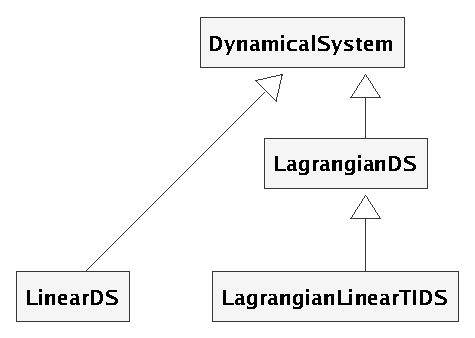
\includegraphics[width=0.3\textwidth]{./DSClassDiagram.eps}
  \label{DSDiagram}
\end{figure}
% DYNAMICAL SYSTEMS
\section{General non linear first order dynamical systems \\ $\rightarrow$ class \it{DynamicalSystem}}
This is the top class for dynamical systems. All other systems classes derived from this one. \\

A general dynamical systems is described by the following set of $n$ equations, completed with initial conditions:
\begin{eqnarray}
  \dot x &=& f(x,t) + T(x) u(x, t) + r \\
  x(t_0)&=&x_0 
\end{eqnarray}

\begin{itemize}
\item $x$: state of the system - Vector of size $n$.
\item $f(x,t)$: vector field - Vector of size $n$.
\item $u(x, t)$: control term - Vector of size $uSize$.
\item $T(x)$: $n\times uSize$ matrix, related to control term.
\item $r$: input due to non-smooth behavior - Vector of size $n$.
\end{itemize}

The Jacobian matrix, $\nabla_x f(x,t)$, of $f$ according to $x$, $n\times n$ square matrix, is also a member of the class. \\

Initial conditions are given by the member $x_0$, vector of size $n$. This corresponds to x value when
simulation is starting, ie after a call to strategy->initialize(). \\

There are plug-in functions in this class for $f$ (vectorField), $jacobianX$, $u$ and $T$. All
of them can handle a vector of user-defined parameters:

% LINEAR DS
\section{First order linear dynamical systems $\rightarrow$ class \it{LinearDS}}

Derived from DynamicalSystem, described by the set of $n$ equations and initial conditions: 
\begin{eqnarray}
  \dot x &=& A(t)x(t)+Tu(t)+b(t)+r \\
  x(t_0)&=&x_0 
\end{eqnarray}
With:
\begin{itemize}
\item $A(t)$: $n\times n$ matrix, state independent but possibly time-dependent.
\item $b(t)$: Vector of size $n$, possibly time-dependent.
\end{itemize}
Other variables are those of DynamicalSystem class. \\
$A$ and $B$ have corresponding plug-in functions. \\

Warning: time dependence for $A$ and $b$ is not available at the time in the simulation part for this kind of dynamical systems. \\

Links with vectorField and its Jacobian are: 
\begin{eqnarray}
  f(x,t) &=& A(t)x(t)+b(t) \\
  jacobianX&=&\nabla_x f(x,t) = A(t) 
\end{eqnarray}

% LINEAR TIDS
\section{First order linear dynamical systems $\rightarrow$ class \it{LinearDS}}

Derived from DynamicalSystem, described by the set of $n$ equations and initial conditions: 
\begin{eqnarray}
  \dot x &=& Ax(t)+Tu(t)+b+r \\
  x(t_0)&=&x_0 
\end{eqnarray}
With:
\begin{itemize}
\item $A(t)$: $n\times n$ constant matrix
\item $b(t)$: constant vector of size $n$
\end{itemize}
Other variables are those of DynamicalSystem class. \\

Links with vectorField and its Jacobian are: 
\begin{eqnarray}
  f(x,t) &=& Ax(t)+b \\
  jacobianX&=&\nabla_x f(x,t) = A
\end{eqnarray}

% LAGRANGIANDS
\section{Second order non linear Lagrangian dynamical systems \\  $\rightarrow$ class \it{LagrangianDS}}

Lagrangian second order non linear systems are described by the following set of$nDof$ equations + initial conditions:
\begin{eqnarray}
 M(q) \ddot q + NNL(\dot q, q) + F_{Int}(\dot q , q , t) &=& F_{Ext}(t) + p \\
 q(t_0) &=& q0 \\
 \dot q(t_0) &=& velocity0 
\end{eqnarray}
With:
\begin{itemize}
\item $M(q)$: $nDof\times nDof$ matrix of inertia.
\item $q$: state of the system - Vector of size $nDof$.
\item $\dot q$ or $velocity$: derivative of the state according to time - Vector of size $nDof$.
\item $NNL(\dot q, q)$:  non linear terms, time-independent - Vector of size $nDof$.
\item $F_{Int}(\dot q , q , t)$: time-dependent linear terms - Vector of size $nDof$.
\item $F_{Ext}(t)$: external forces, time-dependent BUT do not depend on state - Vector of size $nDof$.
\item $p$: input due to non-smooth behavior - Vector of size $nDof$.
\end{itemize}

The following Jacobian are also member of this class:
\begin{itemize}
\item jacobianQFInt = $\nabla_q F_{Int}(t,q,\dot q)$ - $nDof\times nDof$ matrix.
\item jacobianVelocityFInt = $\nabla_{\dot q} F_{Int}(t,q,\dot q)$ - $nDof\times nDof$ matrix.
\item jacobianQNNL = $\nabla_q NNL(q,\dot q)$ - $nDof\times nDof$ matrix.
\item jacobianVelocityNNL = $\nabla_{\dot q}NNL(q,\dot q)$ - $nDof\times nDof$ matrix.
\end{itemize}


There are plug-in functions in this class for $F_{int}$, $F_{Ext}$, $M$, $NNL$ and the four Jacobian matrices. All
of them can handle a vector of user-defined parameters. \\

Links with first order dynamical system are: 
\begin{eqnarray}
  n &= &2nDof \\
  x &=&\left[\begin{array}{c}q \\ \dot q \end{array}\right] \\
  f(x,t) &=&  \left[\begin{array}{c} \dot q \\ M^{-1}(F_{Ext}-F_{Int}-NNL) \end{array}\right] \\
  \\
  \nabla_x f(x,t) &=& 
  \left[\begin{array}{cc} 
      0_{nDof\times nDof} & I_{nDof\times nDof} \\
      \nabla_q(M^{-1})(F_{Ext}-F_{Int}-NNL) -M^{-1}\nabla_q(F_{Int}+NNL) &  -M^{-1}\nabla_{\dot q}(F_{Int}+NNL) 
    \end{array}\right] \\
  r &=& \left[\begin{array}{c} 0_{nDof} \\ p \end{array}\right] \\
  u(x,\dot x,t) &=& u_L(\dot q, q, t) \text{  (not yet implemented)} \\
  T(x) &=& \left[\begin{array}{c} 0_{nDof} \\ T_L(q) \end{array}\right] \text{  (not yet implemented)} \\
\end{eqnarray}
With $0_{n}$ a vector of zero of size $n$, $0_{n\times m}$ a $n\times m$ zero matrix and
$I_{n\times n}$, identity $n\times n$ matrix. \\

Warning: control terms ($Tu$) are not fully implemented in Lagrangian systems. This will be part of future version.

% LAGRANGIAN LINEAR TIME INVARIANT DS
\section{Second order linear and time-invariant Lagrangian dynamical systems $\rightarrow$ class \it{LagrangianLinearTIDS}}

\begin{eqnarray}
M \ddot q + C \dot q + K q =  F_{Ext}(t) + p
\end{eqnarray}

With:
\begin{itemize}
\item $C$: constant viscosity $nDof\times nDof$ matrix 
\item $K$: constant rigidity $nDof\times nDof$ matrix 
\end{itemize}

And: 
\begin{eqnarray}
F_{Int} &=& C \dot q + K q \\
NNL &=& 0_{nDof} 
\end{eqnarray}

\end{document}
